\chapter{Magie}
\section{Das Konzept der Magie}
\subsection{Was ist Magie?}
In diesem Universum ist Magie eine besondere Form der Energie und ist ein Nebenprodukt bei Energieumwandlungen.
Es entsteht also überall dort Magie, wo irgendeine Form der Energie in eine andere umgewandelt wird - was sowohl in der belebten als auch der unbelebten Natur ständig der Fall ist.
So führen z.B. Steinschläge oder Lawinen zu einem plötzlichen Auftreten einer gewissen Menge von Magie, während ein Vulkanausbruch hingegen eine ziemliche Masse an Magie produziert. 
Ja schon allein die Plattentektonik sorgt für das Vorkommen von Magie.
Da Magie eine Form der Energie ist, kann sie deshalb auch selbst wieder zurück in andere Energieformen umgewandelt werden.
Im Allgemeinen "`diffundiert"' die erzeugte Magie nämlich von ihrem Ort der Entstehung hinweg in die Umgebung, da es nichts gibt, was sie halten würde.
Dort wird sie nach und nach wieder umgewandelt.


\subsection{Anpassung der belebten Natur}
Es ist also kein Wunder, dass Magie hier auf \nameref{sec:planet} nichts besonderes ist, und dass sich das Leben dementsprechend auch entwickelte - denn insbesondere in und um Zellen erfolgt am laufenden Band die Umwandlung von Energie zwischen verschiedenen Formen.
Daher haben Zellen eine Möglichkeit entwickelt, Energie in Form von Magie zu halten und zu einem gewissen Grad anzusammeln.
Bei Eukaryoten (Pflanzen, Pilze, Tiere) ist dies eine Art Vakuole. 
Die maximal zu haltende Menge ist artabhängig und angeboren.
Ist diese Menge überschritten, so diffundiert alles Überschüssige wieder aus der Zelle in die Umwelt.
Die so gehaltene Menge an Magie wird auch als Mana oder Manapool bezeichnet.

Eine Verbildlichung lässt sich mit einer Zisterne darstellen: diese füllt sich mit dem Wasser vom Dach des Hauses, bis sie voll ist.
Danach läuft sie über und das Wasser verteilt sich in der Gegend.

Ursprünglich war dies ein Vorteil bezüglich des Überlebens der Zelle: im größten Notfall, wenn die Zelle keine Energiezufuhr jegweder Art erhält, dann kann sie ein energieintensives Notprogramm initialisieren, welches ihr die Magie als tatsächliche Energiereserve zu nutzen ermöglicht.
So kann die Zelle einen kurzen Zeitraum ohne Versorgung überbrücken.
Im Laufe der Evolution haben viele Lebewesen dann Mechanismen entwickelt, um die ihnen innewohnende Magie in ihrem Sinne auf einem intuitiven Level umzuwandeln bzw einzusetzen.
Bei Tieren kann man sich das wie eine Art zweites Nervensystem vorstellen, welches sich an den Adern entlang durch den ganzen Körper zieht und vom Rückenmark aus kontrolliert wird.
Dieses Geflecht wird aus besonderen Zellen gebildet, die selbst keine Magie speichern, sondern die Magie aus den restlichen Zellen des Körpers abziehen.
Diese gelangt somit in das Netzwerk, wo sie über das Rückenmark gezielt kontrolliert werden kann.

In welcher Weise sie die Magie kontrollieren können, ist genetisch festgelegt und hat sich evolutionär entwickelt.
Der Einsatz erfolgt im intuitiven Sinne wie ein Reflex oder eine Reaktion auf etwas, das passiert, oder unterstützt eine Handlung. 
So gibt es Pflanzen, die zur Abwehr von Fressfeinden kleine Elektroschocks verteilen, zum Anlocken von Bestäubern mit Licht spielen, oder Prädatoren, die mittels Infrarot-Magie ihre Beute ohne Probleme von der Umgebung unterscheiden können.

Jeder Mensch beherrscht die Magie auf diesem Level und zeigt sich erstmals im Bereich von 4-7 Jahren.
Im Verlauf der Differenzierungen der verschiedenen Menschenarten haben sich unterschiedliche Ausprägungen durchgesetzt oder sind erst entstanden.


\subsection{Aktive Verwendung}
Einige Lebewesen haben zudem die Fähigkeit entwickelt, die Magie aktiv in ihrem Interesse einzusetzen.
Bei Tieren bedeutet das, dass sich auch das Gehirn bei der Steuerung einschaltet.
Dabei wird sie auf ein Ziel ausgerichtet und dort die bestehenden Zustände geändert.
Es muss allerdings eine deutlich größere Menge an Magie eingesetzt werden, als der Vorgang bzw. die Änderung eigentlich an Energie benötigen würde.
So hat auch der Mensch schließlich festgestellt, dass er mithilfe seines Willens und Konzentration dazu in der Lage ist, diese Möglichkeiten auszubauen und zu verstärken.
Nur Personen, die sich intensiv mit ihren Fähigkeiten auseinandersetzen, viel meditieren, experimentieren und Verständnis suchen, nur diese Personen lernen, das Tauschverhältnis zu reduzieren und immer mehr zu einem halbwegs äquivalenten Austausch zu kommen.
Das führt dazu, dass sie mit dem ihnen angeborenen Manapool mehr und stärkere Dinge bewirken können.
Ihre einzigen Grenzen sind dabei durch ihre Gene, ihre Vorstellungskraft, ihre Konzentrationsfähigkeit und den magischen Widerstand anderer Lebewesen gesetzt. 
\\ \\
Es gibt ein paar Prokaryoten, die sich die Magie als tatsächliche dauerhafte Energiequelle erschlossen haben und sie ständig direkt zur Herstellung von ATP (Adenosintriphosphat = "`Energie der Zelle"') nutzen können.
Bisher ist noch kein Fall von Symbiose oder gar Endosymbiose ähnlich wie mit den Mitos (\textalpha-Proteobakterien $\rightarrow$ Mitochondrien) oder Chloros (Cyanobakterien $\rightarrow$ Chloroplasten) bekannt, aus dem höher entwickelte Lebewesen herausgekommen sind, da dies vor nicht allzu langer Zeit (in Zeiträumen der Evolution) entstand.


\subsection{Natürlicher magischer Widerstand}
Ist es im Allgemeinen nicht schwer, den eigenen Körper und die Umgebung zu beeinflussen, so ist das Verändern von Zuständen in anderen Körpern ein ganz anderes Thema.
Höher entwickelte Lebewesen, die ein Verständnis für den eigenen Körper oder sogar ein Ich-Bewusstsein erstanden haben, besitzen dadurch einen Art natürlichen magischen Widerstand gegen Änderungen, die in ihrem Körper erfolgen sollen. 
Dieser ist umso stärker, je ausgereifter das Bewusstsein ist.
Das führt dazu, dass nur wirklich mächtige und studierte Individuen es schaffen, diese Barriere zu überwinden und Magie innerhalb solcher Körper zu wirken.



\section{Magie-Kontrolle}
\paragraph{Hintergrund}
Magie kann eingesetzt werden, um bestimmte physikalische oder chemische Prozesse zu verändern - in einem gewissen Rahmen, der genetisch vererbt wurde.
Somit bedeutet die Beherrschung einer Magie-Art eigentlich, dass das Wesen dazu fähig ist, die Magie kontrolliert in diese bestimmte Art Energie umzusetzen.
Welche Arten bisher schon entstehen zeigt die kategorisierte Übersicht in Abb. \ref{fig:magiearten-uebersicht}.

\begin{figure}[htb]
	\centering
	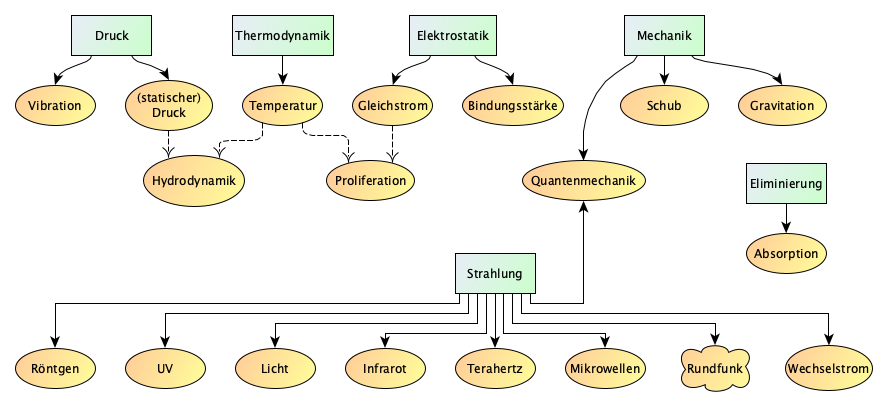
\includegraphics[width=\linewidth]{Abbildungen/Weltenbau/Magie/Magiearten-Uebersicht}
	\caption[Übersicht der Arten der Magiekontrolle]{\textbf{Alle bekannten Arten der Kontrolle über Magie in der Übersicht.} \\ 
	Verwandte Arten sind durch ihre Kategorisierung und ihre Verbindung über Pfeile gekennzeichnet.}
	\label{fig:magiearten-uebersicht}
\end{figure}


\paragraph{Stufen der Kontrolle}
Bei den folgenden verschiedenen Arten der Magie-Kontrolle, auch Magiearten genannt, ist dargestellt, wie die intuitive Nutzung dieser Eigenschaft aussieht oder wie Begabte mit ihr umgehen können.
Meisterliche Magier erreichen noch ganz andere Level. 
In der Regel sind sie schon in hohem Alter und haben sich ihr Leben lang mit der Verbesserung, dem Lernen und Ausprobieren beschäftigt, weshalb es nur wenige von ihnen gibt, die so weit kommen. 
Neben der Intensivierung und Verbesserung vorheriger Zauber gelingt ihnen auch eine Manipulation ganz anderer Art: 
Sie können die natürliche Resistenz des Körpers (siehe oben) umgehen.


\paragraph{Magie-Arten}
Die Informationen über die Verbreitung der Magiearten unter den Lebewesen und ihrer Bekanntheit in \nameref{sec:land} finden sich einerseits bei jeder Art und andererseits in Tab. \ref{tab:magie-verbreitung} zur Übersicht.

Die Anordnung der Magiearten ist alphabetisch, um einen schnellen Zugriff zu ermöglichen.

\begin{table}[htb]
	\centering
	\caption{\textbf{Verbreitung der Magiearten unter den Lebewesen allgemein und unter den Menschenarten.}}
	\label{tab:magie-verbreitung}
	\begin{threeparttable}[\linewidth]
		\begin{tabularx}{\textwidth}{l|ccc}
			\toprule
			\textbf{Art} & \textbf{Eukaryoten} & \textbf{Hominini} & \textbf{Mensch} \\
		    \midrule
			\nameref{sec:nullmagie}  & - & - & (x)  \\
			\nameref{sec:bindungsmagie} & X & \nameref{rasse:sylvan} & -  \\
			(statischer) \nameref{sec:druckmagie} & X & X & X  \\
			\nameref{sec:gleichstrommagie}  & X & X & X  \\
			\nameref{sec:gravitationsmagie} & - & - & - \\ \midrule[0.1px]
			\nameref{sec:hydrodynamikmagie} X & X & X &\\
			\nameref{sec:infrarotmagie} & X & & \\
			\nameref{sec:lichtmagie}  & X & X & X  \\
			\nameref{sec:mikrowellenmagie} & X & &\\
			\nameref{sec:proliferationsmagie} & X & X & X \\ \midrule[0.1px]
			\nameref{sec:quantenmechanikmagie} & X & ? & - \\
			\nameref{sec:roentgenmagie} & X & - & - \\
			\nameref{sec:rundfunkmagie} & X & - & - \\
			\nameref{sec:schubmagie} & X & X & \\
			\nameref{sec:temperaturmagie} & X & X & X  \\ \midrule[0.1px]
			\nameref{sec:terahertzmagie} & X & & \\
			\nameref{sec:uvmagie} & X & \nameref{rasse:ferus} & ggf. \\
			\nameref{sec:vibrationsmagie} & X & \nameref{rasse:zwerg}, \nameref{rasse:unda} & -  \\
			\nameref{sec:wechselstrommagie} & X & X & X \\
			\bottomrule
		\end{tabularx}
	\end{threeparttable}
\end{table}



\subsection{Absorption oder Nullmagie}\label{sec:nullmagie}
Diese Art der Kontrolle sorgt für einen ständigen Entzug von Magie aus der Umwelt, da zumindest beim Menschen die eigenen Zellen nicht mehr fähig sind, diese zu halten und somit versuchen, auszugleichen. 

\subsubsection{Verbreitung und Bedeutung im Spiel}
Zu Beginn des Spiels beherrschen nur Mikroorganismen diese Fähigkeit. Sie ist daher anfangs vollkommen unbekannt. 
Am Ende des Spiels wird eine neue Art Mensch geschaffen, die diese Fähigkeit ebenso beherrschen.

\subsubsection{Intuitive Nutzung}
Die Bakterien nutzen es als Energiequelle mittels eines speziellen Zellorgans. 
Es lässt sich ähnlich vorstellen wie die Nutzung von Sonnenenergie mittels Chloroplasten oder chemischer Energie mittels Mitochondrien. 

Die Menschen werden durch das heftige Ziehen sämtlicher Magie relativ unbeeinflussbar durch Magie, die direkt auf sie gewirkt wird oder auf das, was sie berühren. 
Sie sind jedoch unfähig, selbst Magie zu wirken.

\subsubsection{Erlernbare Steigerungen}
Es wird sehr lange dauern, bis die Menschen begreifen, dass auch dies eine Möglichkeit zur Steigerung bietet.
\begin{outline}
	\1 Magie, die gerade auf die erweiterte Umgebung gewirkt wird, wird annulliert.
	\1 Es ist ein verlängertes Fasten möglich, da der Körper auf die Umgebungsmagie zurückgreift.
	\1 ...
\end{outline}

\subsubsection{Meisterliche Beherrschung} 
\begin{outline}
	\1 Aktives Absorbieren von Magie aus Lebewesen, was diese daran hindert, ihre Magie einsetzen zu können.
	\1 ...
\end{outline}
Zurück zu Tab. \ref{tab:magie-verbreitung}.



\subsection{Bindungsstärke}\label{sec:bindungsmagie}
Mittels dieser Fähigkeit lassen sich Atombindungen stärken oder schwächen, wodurch ein Verhärtungs- oder Erweichungseffekt hervorgerufen wird. 
Allerdings führt eine höhere Bindungsenergie auch zu einer kleineren räumlichen Nähe der Atome. 
Da die Magie der Bindungsstärke erst unter Einfluss der \nameref{sec:druckmagie}-Magie entstand, wird dabei gleichzeitig ein starker negativer (Verhärtung) oder positiver (Erweichung) Druck von außen appliziert. 
Dadurch verkleinert oder vergrößert sich das veränderte Material nicht plötzlich um den gleichen Faktor.

\subsubsection{Verbreitung}
Dies ist vor allem unter Pflanzen, wie auch den Bäumen aus dem \nameref{sec:gigantuswald}, verbreitet.
Bei den Hominini können nur Sylvan auf diese Weise Magie kontrollieren.

\subsubsection{Bedeutung im Spiel}
Derzeit ist keine Bedeutung im Spiel geplant. 
Eventuell durch andere Lebewesen oder sollte man die Sylvan (ggf. auch durch ein DLC) tatsächlich treffen können.

\subsubsection{Intuitive Nutzung}
Intuitiv nutzen Lebewesen dies, um den eigenen Körper zu stärken, wenn es um eingehende Verletzungen geht, zB. beim Kampf oder beim Fallen (Schockabsorption). 
Einige machen ihren Körper dadurch zeitweise etwas beweglicher, um durch kleinere Spalte hindurch zu passen.
Dies ist auch anwendbar auf Oberflächen, die direkt berührt werden. 
Auf diese Art sorgen zB. die Sylvan dafür, dass sie auch bei etwas dünneren Blättern oder Ästen nicht durch krachen.

\subsubsection{Erlernbare Steigerungen}
\begin{outline}
	\1 Zerreißen von Dingen.
	\1 Extremes Erhärten von Luft, um sie als stabile Wand zu nutzen.
	\1 Bewusstes Weglassen des Drucks von außen führt zu einer Volumenänderung des betroffenen Bereichs. 
	Dies bedeutet einerseits starkes Anwachsen oder extremes Verkleinern. 
	Das Gewicht ändert sich dabei nicht. 
	Die Weiterleitung von Signalen an Nervenzellen u.ä. ist allerdings auch beeinträchtigt: wenn größer, dann langsamer, wenn kleiner, dann schneller.
	\1 ...
\end{outline}

\subsubsection{Meisterliche Beherrschung} 
\begin{outline}
	\1 Erschaffen temporärer Löcher im Körper, durch die zB etwas durch kann, bevor dies wieder rückgängig gemacht wird.
	\1 Anwendung in Alchemie: Stoffe werden dazu gebracht Verbindungen einzugehen, die normalerweise eine zu hohe Energiebarriere haben.
	\1 ...
\end{outline}
Zurück zu Tab. \ref{tab:magie-verbreitung}.



\subsection{Druck}\label{sec:druckmagie}
Diese Eigenschaft erlaubt die Kontrolle über den lokalen, statischen Druck. 
Es existiert die präzisere Unterform \nameref{sec:vibrationsmagie}, sowie die Neuentwicklung der Magie der \nameref{sec:bindungsmagie}.

\subsubsection{Verbreitung}
Ähnlich wie bei der thermischen Energie ist diese Form recht weit verbreitet. 
Die homininen Arten beherrschen diese Kontrolle. 

In unserem Land ist die Magieform allerdings nicht ganz so häufig wie die der Temperatur anzutreffen. 
Ansonsten ist sie gut bekannt.

\subsubsection{Bedeutung im Spiel}
Die \npref{sec:mc-diplomatin} hat diese Eigenschaft ab ihrem Schlüsselmoment. %todo

\subsubsection{Intuitive Nutzung}
Die Lebewesen können somit in einer Art Reaktion Gefahren, die zu nah an sie herankommen, von sich wegschubsen, ohne sie zu berühren, oder sich selbst aus einem gefährlichen Bereich heraus drängen. 

\subsubsection{Erlernbare Steigerungen}
\begin{outline}
	\1 Es sind deutlich weitere und höhere Sprünge möglich.
	\1 Es wird Druck auf andere Dinge angewendet, womit sie entweder auseinander gerissen oder zerquetscht werden.
	\1 Gegenstände oder Lebewesen werden kontrolliert an Ort und Stelle gehalten oder durch die Gegend gedrückt.
	\1 Der eigene Körper kann etwas über den Boden schweben.
	\1 Einkommender Druck kann abgefangen und auf eine größere Fläche verteilt werden: zuerst nur bei größerflächigen Dingen wie Steinen oder Stöcke. 
	Später auch gegen Waffen, die genau so was ausnutzen: Klingenwaffen. 
	Dadurch wird weniger Schaden genommen.
	\1 ...
\end{outline}

\subsubsection{Meisterliche Beherrschung} 
\begin{outline}
	\1 Den Druck im Kopf erhöhen, bis er platzt.
	\1 Den Blutdruck plötzlich extrem absenken, so dass der Gegenüber bewusstlos zusammenbricht. 
	\1 Den Druck in der Umgebung so stark beeinflussen, dass sich dadurch das Wetter ändern kann. Damit lassen sich zB. Regenwolken lenken. 
	\1 Eine Art Fliegen, aber mehr im Sinne eines erweiterten Schwebens.
	\1 ...
\end{outline}
Zurück zu Tab. \ref{tab:magie-verbreitung}.



\subsection{Gleichstrom}\label{sec:gleichstrommagie}
Mit dieser Eigenschaft lassen sich elektrische Ladungen beeinflussen und verschieben.
So kann eine große Potentialdifferenz zwischen zwei Orten aufgebaut werden, die sich ab einem bestimmten Punkt selbst ausgleicht: meist in Form eines Blitzes.
Weiterhin ist es mit dieser Beeinflussung möglich, die nötige Ladung so zu verschieben, dass Redox-Reaktionen ablaufen: Funken fliegen, Feuer entsteht, Explosionen krachen.

\subsubsection{Verbreitung}
Dies ist weit unter Tieren und insbesondere Pflanzen verbreitet. 
Doch auch die Hominini besitzen diese Fähigkeit, allerdings ist ihnen Elektrizität im weiteren (heutigen) Sinne noch kein Begriff, weshalb das bisherige Ausnutzen und Ausbauen dieser Kontrolle recht schlecht erforscht ist.
Meist beschränkt es sich auf das Auslösen von Reaktionen.

\subsubsection{Bedeutung im Spiel}
Die \npref{sec:mc-diplomatin} erhält den Zugriff auf diese Fähigkeit nach ihrem Schlüsselerlebnis. 

\subsubsection{Intuitive Nutzung}
Da die Weiterleitung von elektrischen Impulsen an Nerven dem Prinzip des Gleichstroms folgt, ist dies bei den Besitzern beschleunigt.
Daraus folgt eine etwas schnellere körperliche Reaktion auf Situationen.
Zudem schweben die anwendenden Lebewesen durch einen Blitzeinschlag nicht in Lebensgefahr.  

\subsubsection{Erlernbare Steigerungen}
\begin{outline}
	\1 Es kann ein Potentialunterschied zwischen zwei Punkten hergestellt werden, der zu einem Ausgleich der Energie über einen Blitz führt.
	Die Stärke des Blitzes und die Entfernung der Punkte a) zueinander und b) vom Anwender sind von dessen Fähigkeiten abhängig.
	Zu Beginn wird nur eine Übertragung zwischen sich und einem anderen Punkt möglich sein.
	\1 Entflammbare Objekte können angezündet werden, da der Reaktion zwischen Objekt und dem Sauerstoff aus der Luft der nötige Schubs zum Start gegeben wird.
	\1 Mit der nötigen Energiemenge lässt sich das Wasser in der Luft in Sauerstoff und Wasserstoff spalten und somit Knallgas herstellen.
	Kommt das Knallgas mit einem Funken in Kontakt, führt das zu einer sofortigen explosiven Revers-Reaktion, bei der sich die beiden wieder zu Wasser verbinden.
	Einflüsse, Stellschrauben u.ä. für die Erweiterung dieses Skills zur Anwendung im Spiel finden sich \zB auf \href{https://de.wikipedia.org/wiki/Knallgas}{Wikipedia}.
	\1 ...
\end{outline}

\subsubsection{Meisterliche Beherrschung} 
\begin{outline}
	\1 Der elektrische Signalfluss an Nervenzellen lässt sich stören, womit zum Beispiel eine Reaktion des Gegenübers verhindert wird. 
	Das ist allerdings recht unpräzise, da die Funktionsweise des Körpers noch nicht so weit bekannt ist. 
	Durch das Spüren der Ströme konnten allerdings einige Erkenntnisse gewonnen werden. 
	So lässt sich \zB sämtlicher elektrischer Fluss in einzelne Gliedmaßen ausschalten, wodurch diese nicht mehr bewegt werden können.
	\1 Ebenso kann man das Gehirn von jemanden lahm legen und ihn damit effektiv töten.
	\1 Das Herz wird von einem Nervenknoten, dem Sinus, kontrolliert. 
	Bei Herzstillstand kann man es wieder zum schlagen bringen, indem man diesem Knoten einen elektrischen Impuls gibt, damit das Herz wieder zu arbeiten beginnt (siehe auch \href{https://de.wikipedia.org/wiki/Defibrillator}{Defibrillator}).
	\1 Schnelleres Denken.
	\1 ...
\end{outline}
Zurück zu Tab. \ref{tab:magie-verbreitung}.



\subsection{Gravitation}\label{sec:gravitationsmagie}
Diese Magieform erlaubt eine Beeinflussung der Gravitation.

\subsubsection{Verbreitung}
Dies ist eine äußerst seltene Magieform, die von keinen bisher bekannten Tieren oder Pflanzen verwendet wird.
Auch unter den Hominini ist sie nicht verbreitet.

\subsubsection{Bedeutung im Spiel}
Derzeit keine Bedeutung im Spiel.

\subsubsection{Intuitive Nutzung}
Intuitiv kann man damit die Auswirkung der Gravitation auf sich selbst reduzieren, was u.a. zu deutlich höheren und weiteren, aber auch unpräziseren Sprüngen führt.

\subsubsection{Erlernbare Steigerungen}
\begin{outline}
	\1 Durch Erhöhen der Gravitation in einem Bereich lassen sich dort andere Lebewesen festhalten.
	\1 Anders herum kann man so auch befreundeten Wesen beim Springen oder ähnlichem helfen.
	\1 ...
\end{outline}

\subsubsection{Meisterliche Beherrschung} 
\begin{outline}
	\1 Durch Wirken von Gravitation im Körper von anderen, lässt sich damit ihr Innenleben zerreißen und verzerren, weshalb sie wahrscheinlich einen sehr schmerzhaften Tod sterben.
	\1 ...
\end{outline}
Zurück zu Tab. \ref{tab:magie-verbreitung}.



\subsection{Hydrodynamik}\label{sec:hydrodynamikmagie}
Hier geht es  um Strömungen von Flüssigkeiten und Gasen.
Am verständlichsten sollte dies sein, wenn von Wind oder Wasserströmen gesprochen wird.
Die Kontrolle über Hydrodynamik entsteht aus einem Mix der Fähigkeiten von \nameref{sec:druckmagie} und \nameref{sec:temperaturmagie}, da sie so erzeugt werden kann.

\subsubsection{Verbreitung}
An sich ist dies eine durchaus verbreitete Magieart unter den Lebewesen.

\subsubsection{Bedeutung im Spiel}
Dies ist eine Fähigkeit, die normal unter der Bevölkerung verbreitet ist.

\subsubsection{Intuitive Nutzung}
Lebewesen können damit direkt um sich herum Wind erzeugen oder diesen negieren und sind daher von stürmischen Auswirkungen meist weniger betroffen.

Menschen lassen dabei auch bei Windstille diesen gerne mal mit ihren Haaren oder der Kleidung spielen.

\subsubsection{Erlernbare Steigerungen}
\begin{outline}
	\1 Das Erzeugen kleiner Windhosen bzw. Staubteufel bzw. Verwirbelungen im Wasser.
	\1 Ein wenig "`Wasserbändigen"'.
	\1 ...
\end{outline}

\subsubsection{Meisterliche Beherrschung} 
\begin{outline}
	\1 "`Blutbändigen"'.
	\1 Erzeugen von Wirbelstürmen.
	\1 ...
\end{outline}
Zurück zu Tab. \ref{tab:magie-verbreitung}.



\subsection{Infrarot}\label{sec:infrarotmagie}
Infrarot-Strahlung ermöglicht das Sehen von Temperatur. 
Die ist bereits in Tieren natürlich entstanden, doch einige nutzen für den gleichen Zweck die Magie.

\subsubsection{Verbreitung}
Nur Tiere haben diese Fähigkeit entwickelt, auch ein paar Menschenstämme in extremen Temperaturgebieten.
% Menschen sind auch Tiere. Pflanzen, Pilze und Mikroorganismen sind damit aber ausgeschlossen.

\subsubsection{Bedeutung im Spiel}
Derzeit keine Bedeutung im Spiel geplant außer über Tiere.

\subsubsection{Intuitive Nutzung}
Tiere auf der Jagd, der Lauer oder beim Wachdienst nutzen eine regelmäßige Überprüfung der Umgebung mittels Infrarotstrahlung, um die wärmeren Körper ihrer Ziele zu sehen.


\subsubsection{Erlernbare Steigerungen}
\begin{outline}
	\1 In besonders kalten Gegenden hat es zu einem gegenseitigen Wettrennen zwischen Jäger und Beute geführt, bei der der Jäger die Beute mittels dieser Sicht aufspüren will, während diese damit die Abgabe ihrer Körperwärme überdeckt.
	\1 Das Erzeugen von "`falschen"' Wärmebildern, indem an anderen Orten Infrarotstrahlung erzeugt wird.
	So kann \zB ein Jäger auf die falsche Fährte geführt werden.
	\1 ...
\end{outline}

\subsubsection{Meisterliche Beherrschung} 
\begin{outline}
	\1 ...
\end{outline}
Zurück zu Tab. \ref{tab:magie-verbreitung}.



\subsection{Licht und Dunkelheit} \label{sec:lichtmagie}
Diese Eigenschaft ermöglicht die Kontrolle von Licht bzw. dessen Abwesenheit.

\subsubsection{Verbreitung}
Eine recht weit verbreitete Kontrollfähigkeit unter Lebewesen. 
Bei den Hominini ist sie nicht so stark verbreitet wie andere.

\subsubsection{Bedeutung im Spiel}
Die \npref{sec:mc-spionin} beherrscht diese Eigenschaft. 

\subsubsection{Intuitive Nutzung}
Viele Lebewesen nutzen dies zur Attraktion von anderen Lebewesen, sei es um diese zu Nutzen oder als Beute. Einerseits Licht insbesondere bei Nacht, andererseits Illusionen um zu täuschen. \\
Man munkelt auch von einer Tierart, die sich so gut an die Umwelt anpassen, dass sie von ihrer Beute nicht entdeckt wird, bis es zu spät ist. 

Menschen nutzen dies besonders um sich selbst attraktiver zu machen, können aber kein Licht selbst erzeugen.

\subsubsection{Erlernbare Steigerungen}
\begin{outline}
	\1 Das Erzeugen von Licht.
	\1 Mit hellem Licht lassen sich Gegner blenden oder gar erblinden.
	\1 Illusionen dienen zur Unterhaltung oder Ablenkung.
	\1 Mittels Illusionen kann man sich dem Hintergrund anpassen, wodurch man deutlich schlechter zu sehen ist.
	\1 ...
\end{outline}

\subsubsection{Meisterliche Beherrschung} 
\begin{outline}
	\1 Wahre Meister des Fachs können das Licht so geschickt manipulieren, dass sie einem unaufmerksamen Auge gar als unsichtbar scheinen können.
	\1 Die Kontrolle über die An- oder Abwesenheit von Licht in einem gewissen Bereich.
	\1 ...
\end{outline}
Zurück zu Tab. \ref{tab:magie-verbreitung}.



\subsection{Mikrowellen}\label{sec:mikrowellenmagie}
Mit Mikrowellen lässt sich Wasser erhitzen und abkühlen, denn diese treffen genau die Eigenfrequenz des Wassers.
Das gilt demnach für alles, was Wassermoleküle enthält.
Weiterhin ermöglichen Mikrowellen ein Radarsystem.

\subsubsection{Verbreitung}
Vor allem Tiere.

\subsubsection{Bedeutung im Spiel}
...

\subsubsection{Intuitive Nutzung}
Viele Tiere mit dieser Eigenschaft haben parallel ein Radarsystem entwickelt.
Die Sensoren befinden sich mit bei den Ohren.
Das erlaubt Herdentieren oder Rudel, sich auch über weitere Strecken hinweg zu lokalisieren, wiederzufinden oder in Bezug auf Beute zu wissen, in welche Richtung ihr noch niemand auflauert.

\subsubsection{Erlernbare Steigerungen}
\begin{outline}
	\1 ...
\end{outline}

\subsubsection{Meisterliche Beherrschung} 
\begin{outline}
	\1 ...
\end{outline}
Zurück zu Tab. \ref{tab:magie-verbreitung}.



\subsection{Proliferation}\label{sec:proliferationsmagie}
Diese Eigenschaft ist eher chemischer Natur und erlaubt die Beeinflussung der Reaktionsgeschwindigkeit.
Aus diesem Grunde leitet sie sich auch von der \nameref{sec:temperaturmagie} und dem \nameref{sec:gleichstrommagie} ab.
Ersteres hat direkten Einfluss auf die Geschwindigkeit: bei erhöhter Temperatur laufen Reaktionen schneller ab, da sich Teilchen schneller bewegen.
Der Gleichstrom dient als Katalysator und senkt die Energiebarriere die dem Start der Reaktion entgegensteht.
Folgen von beschleunigten Reaktionen findet sich dann auch bei den Zellen wieder: schnelleres Wachstum führt zum Beispiel zu einem schnelleren Lebenszyklus oder zur beschleunigten Reparatur von Schäden - auch im gesamten Gewebe.

\subsubsection{Verbreitung}
Wenige Pflanzen- und Tierarten sind dieser Fähigkeit mächtig. 
Auch bei den Hominini ist es eine seltene Gabe. 
Denn diese Fähigkeit leitet sich zwar von den recht häufig verbreiteten Arten Temperatur und Gleichstrom ab, doch nicht immer, wenn im Nachfahren diese Kombination vorliegt, beherrscht dieser die Proliferation.
Daher ist sie so selten und hoch geschätzt.
Diese Hominini leben länger als ihre Verwandten, abhängig von der Intensität ihrer Begabung sogar bis zu \SI{200}{\percent} der durchschnittlichen Lebensdauer.
Allerdings kommt mit dieser Fähigkeit ein ungünstiger Nachteil: sie sind unfähig, sich mit ihren Artangehörigen zu vermehren, da ihre Keimzellen "`nicht auf gleicher Geschwindigkeit laufen"'.

\subsubsection{Bedeutung im Spiel}
Nur sehr wenig Individuen im Land haben diese Kontrollform geerbt.
Insbesondere begabte Menschen, die zur aktiven Anwendung außerhalb des eigenen Körpers fähig sind, bleiben Einzelbeispiele.
Diese sind daher hochgeschätzte Mitglieder des Ordens und erfreuen sich besten Umständen.

Es heißt, es liegt ein solcher Magier irgendwo in einer Art Winterschlaf und er wird aufwachen, wenn die Welt ihn wieder benötigt (Ref: wie die Sage zu König Barbarossa? Ggf. unter Märchen und Quests ausfeilen). %todo

\subsubsection{Intuitive Nutzung}
Da Reparatur und Heilung schneller ablaufen, sich der Körper ansonsten aber "`ruhiger verhält"', verläuft der Alterungsprozess langsamer.

\subsubsection{Erlernbare Steigerungen}
\begin{outline}
	\1 Erweitern der gesteigerten Reaktionen auf die nahe Umwelt: Pflanzen wachsen und reifen schneller.
	\1 Zudem kann dies zur Heilung anderer eingesetzt werden, wenn diese ihre natürliche Resistenz senken.
	Diese ist durch eine bestimmte Droge umgehbar, welche allerdings auch zusätzliche Belastung auf den Körper auswirkt. %todo ein schöner Ansatzpunkt für Folter und den Geheimdienst
	Das führt dazu, dass manche schwere Verletzungen nicht geheilt werden können, weil schon die Einnahme der Droge den Körper überstrapaziert.
	\1 ...
\end{outline}

\subsubsection{Meisterliche Beherrschung} 
Nur extrem wenige Menschen haben es geschafft, diese Stufe zu erreichen.
Sie sind daher geliebte und gefürchtete Individuen.
\begin{outline}
	\1 Das plötzliche starke Altern des Gegenübers.
	\1 Krebserzeugung.
	\1 ...
\end{outline}
Zurück zu Tab. \ref{tab:magie-verbreitung}.



\subsection{Quantenmechanik}\label{sec:quantenmechanikmagie}
Dies ist eine experimentelle Magieform, die wahrscheinlich keinem normalen Lebewesen zur Verfügung steht.
Ein wenig ist das die Form, die am Meisten an die klassische OP-Magie mit Teleportation, Verdopplung etc. heranreicht.
Demzufolge braucht sie allerdings auch die meiste Energie - und zwar in so gigantischen Ausmaßen, dass sie teilweise nicht annähernd vernünftig zu erklären wäre.
So bräuchte die Teleportation eines Menschen schon etwa die Energiemenge einer ganzen Galaxie...

\subsubsection{Bedeutung im Spiel}
Derzeit keine Bedeutung im Spiel.

\subsubsection{Ausnutzen der Quantenmechanik}
\begin{outline}
	\1 Welle-Teilchen-Dualismus
		\2 Teilchen können sich auch wie Wellen verhalten und deshalb mit sich selbst interferieren.
		\2 Interpretation: es lassen sich einige Eigenschaften des eigenen Körpers verbessern, während sich dafür andere Verschlechtern.
		Also ein Buff zum Preise eines Debuffs.
	\1 Tunnelrate
		\2 Ein Teilchen befindet sich nur an seinem Platz, weil ihm die Energie fehlt, an einem anderen zu sein.
		\2 Interpretation: Teleportation.
	\1 Superposition
		\2 Teilchen können in mehreren Zuständen gleichzeitig existieren.
		\2 Interpretation: Duplikation von Dingen, ggf. erneute Verschmelzung nach bestimmter Zeit.
\end{outline}
Zurück zu Tab. \ref{tab:magie-verbreitung}.



\subsection{Röntgen}\label{sec:roentgenmagie}
Röntgenstrahlung erlaubt es, tief in organisches Material hineinzusehen. 

\subsubsection{Verbreitung}
Einige Tiere beherrschen diese Fähigkeit. \\
Keine Verbreitung unter den Hominini.

\subsubsection{Bedeutung im Spiel}
Derzeit keine Bedeutung im Spiel.

\subsubsection{Intuitive Nutzung}
Gerade Jäger, die ihre Beute unter Deckung wie Felsen oder Erde suchen, nutzen kurze blitzartige Momente der Röntgenstrahlung, um ihre Beute zu lokalisieren.
Da diese Strahlung sehr energieintensiv ist, ist eine häufige Anwendung mit dem normalen Pool an Mana nicht möglich.
\\ \\
Zurück zu Tab. \ref{tab:magie-verbreitung}.



\subsection{Rundfunk}\label{sec:rundfunkmagie}
Diese Wellenlänge wird heutzutage zum Rundfunk genutzt.
Uns ist nichts eingefallen, wie man dies als Fähigkeit für eine nicht-technologisierte Welt einsetzen könnte.
Denn den Wesen einfach einen (detaillierten) Interpreter und Sender wie bei unseren Radiostationen in den Kopf zu packen, erschien uns unlogisch.
Da diese Frequenzen aber mitten drin unter den anderen genutzten liegt, ist eine Evolution dieser Fähigkeit äußerst wahrscheinlich.
Daher behalten wir sie uns als Option drin, insbesondere für eine spätere Nutzung im entsprechenden Zeitalter.

Sollte jemand sich mit der Thematik des Rundfunks besser auskennen und doch dafür plädieren (und es damit als eine Art Telepathie einsetzen wollen), dann bitte zur Diskussion melden.

\subsubsection{Verbreitung}
Keine Verbreitung unter den Lebewesen.

\subsubsection{Bedeutung im Spiel}
Derzeit keine Bedeutung im Spiel.
\\ \\
Zurück zu Tab. \ref{tab:magie-verbreitung}.



\subsection{Schub}\label{sec:schubmagie}
Schub steht für die mechanische Energie, die auf etwas appliziert werden kann.
Diese Magieart entspricht damit dem Bild einer erweiterten Hand, die diese Kraft ausübt.


Zur Unterscheidung von \nameref{sec:druckmagie} kann man sich hier vor Augen halten, dass der Druck auf alles an der entsprechenden Stelle gilt, da er außerhalb angesetzt wird (das kann auch Auswirkungen auf das Objekt selbst haben!). 
Die mechanische Kraft wirkt jedoch nur auf ein bestimmtes Objekt.
Damit sind bei ähnlichen Anwendungen präzisere Ausführungen möglich.
Zudem kann je nach Umstand der Druck an seine Grenzen kommen, wo die mechanische Kraft noch keine Grenzen hat.

Weiterhin unterscheidet sie sich vom Druck darin, dass es immer um eine Bewegung geht.
Kann mittels Druck etwas zerquetscht werden, so ist dies mit Schub nicht möglich: dazu müsste man andere Dinge nehmen, die den Schub Richtung des zu Zerquetschendes erhalten.

\subsubsection{Verbreitung}
Eine normale, weit verbreitete Fähigkeit.

\subsubsection{Bedeutung im Spiel}
Eine normale Fähigkeit unter der Bevölkerung.

\subsubsection{Intuitive Nutzung}
Ideen pls.

\subsubsection{Erlernbare Steigerungen}
\begin{outline}
	\1 Levitation
	\1 Telekinese
	\1 ...
\end{outline}

\subsubsection{Meisterliche Beherrschung} 
\begin{outline}
	\1 Herumschieben von anderen Personen.
	\1 ...
\end{outline}
Zurück zu Tab. \ref{tab:magie-verbreitung}.



\subsection{Temperatur}\label{sec:temperaturmagie}
Diese Eigenschaft erlaubt die Kontrolle über die thermische Energie der Umgebung, sowohl das Erhitzen als auch das Abkühlen.

\subsubsection{Verbreitung}
Diese Manipulation der thermischen Energie ist uralt und daher weit verbreitet unter allen Arten von Lebewesen; Somit auch unter den homininen Arten. 
Sie ist gut bekannt.

\subsubsection{Bedeutung im Spiel}
Diese Magiekontrolle beherrscht der \npref{sec:mc-soldat}. Es ist ansonsten eine der am weitesten verbreiteten Arten unter der Bevölkerung.

\subsubsection{Intuitive Nutzung}
Diese Lebewesen haben weniger Temperaturprobleme, da sie den Temperaturaustausch mit der Umgebung reduzieren können.
Einige Tiere nutzen dieses Konzept auch zur Jagd, sowohl an Land als auch im Wasser, wo sie die Luft oder das Wasser stark erhitzen oder extrem abkühlen und damit für Verbrennungen oder Erfrierungen sorgen.

\subsubsection{Erlernbare Steigerungen}
Zuerst Beispiele für die Erhitzung:
\begin{itemize}
	\item Das Erhitzen von Gegenständen abseits vom eigenen Körper, insbesondere sehr gut Wärme-leitenden Materialien wie Metall. Dies wird zB. im Kampf ausgenutzt, um die Waffe oder die Rüstung des Gegners zu heiß zum Halten/Tragen werden zu lassen.
	\item Das Entzünden entflammbarer Objekte.
	\item Das Erschaffen kleiner Massen glühender Hitze, die weggeworfen werden kann. Beim Aufprall entzünden sich die vor Ort befindlichen Materialien. 
	\item Wandförmige Bereichen von Luft werden so stark erhitzt, dass alles, was sie berührt, schmilzt oder brennt.
	\item ...
\end{itemize}

Nun Beispiele für das Abkühlen:
\begin{itemize}
	\item Das Metall am Körper des Gegenübers erkalten lassen. Das kann zu Verbrennungen führen.
	\item Feuchte Körperteile lassen sich an gefrorenen Gegenständen, insbesondere metallischen, anfrieren.
	\item Flüssigkeiten auf dem Boden (idR Wasser) lassen sich gefrieren, womit Glatteis erzeugt wird.
	\item Feuer lassen sich durch einen gegensätzlichen Effekt löschen.
	\item ...
\end{itemize}

\subsubsection{Meisterliche Beherrschung} 
\begin{itemize}
	\item Das Blut/der Körper des Gegners kann zum Kochen gebracht werden.
	\item Körperteile des Gegners können erfroren werden.
	\item ...
\end{itemize}
Zurück zu Tab. \ref{tab:magie-verbreitung}.



\subsection{Terahertz}\label{sec:terahertzmagie}
Mittels Terahertz-Strahlung lässt sich wenige Zentimeter in weiches bzw. organisches Gewebe blicken, ohne Strahlungsschäden zu riskieren.
Diese Wellenlänge wird allerdings schon von Wasser absorbiert.
Das erklärt die geringe Reichweite und Unschädlichkeit.

\subsubsection{Verbreitung}
Gerade unter den intelligenteren Tieren verbreitet, aufgrund des guten intuitiven Nutzens.

\subsubsection{Bedeutung im Spiel}
Je nachdem inwiefern es den Menschen in Mantodea zur Verfügung steht. %todo

\subsubsection{Intuitive Nutzung}
Diese Fähigkeit ermöglicht es, sehr schnell Parasiten zu finden oder sich der genaueren Natur einer Verletzung gewahr zu werden.

\subsubsection{Erlernbare Steigerungen}
\begin{outline}
	\1 ...
\end{outline}

\subsubsection{Meisterliche Beherrschung} 
\begin{outline}
	\1 ...
\end{outline}
Zurück zu Tab. \ref{tab:magie-verbreitung}.



\subsection{UV}\label{sec:uvmagie}
Es gibt Tiere, die bereits im UV-Spektrum sehen können, ohne über Magie zu verfügen. 
Darunter fällt die Biene.

\subsubsection{Verbreitung}
Gerade Pflanzen nutzen dies, um attraktiver für Bestäuber wirken zu können. \\
Die \nameref{rasse:ferus} nutzen dies, um auch unter der Erde Vitamin~D herstellen zu können.

\subsubsection{Bedeutung im Spiel}
Derzeit keine Bedeutung im Spiel.

\subsubsection{Intuitive Nutzung}
Tiere nutzen das \zB anstatt der normalen Sicht oder ähnlich wie Bienen.

Die \nameref{rasse:ferus} hingegen erzeugen immer wieder kleine Mengen UV-Strahlung in ihrer Haut, wodurch sie auch unter der Erde dazu in der Lage sind, das nötige Vitamin~D herzustellen.

\subsubsection{Erlernbare Steigerungen}
\begin{outline}
	\1 ...
\end{outline}

\subsubsection{Meisterliche Beherrschung} 
\begin{outline}
	\1 ...
\end{outline}
Zurück zu Tab. \ref{tab:magie-verbreitung}.



\subsection{Vibration}\label{sec:vibrationsmagie}
Diese Fähigkeit ist eine Weiterentwicklung der \nameref{sec:druckmagie} im Sinne einer präziseren Manipulation.\\
Der Körper ist dazu in der Lage, verschieden-frequentige Vibrationen zu erzeugen. 
Häufig ging daher auch eine Evolution von feineren Sinnesorganen zur Rezeption dieser damit einher.

\subsubsection{Verbreitung}
Manche Lebewesen kontrollieren Magie auf diese Art, darunter auch die \nameref{rasse:zwerg} und \nameref{rasse:unda} der homininen Arten. Die Menschen beherrschen diese Verwendung der Magie nicht und da eine Reproduktion mit den anderen Arten nach der ersten Generation in einer Sackgasse steckt, bleibt ihnen nur die Erforschung.

\subsubsection{Bedeutung im Spiel}
Bedeutung findet sich hier keine weitere für die Menschen des Landes, nur in der Forschung. 
Bei den paar Zwergen, die unter den Menschen leben, sieht das natürlich anders aus.

\subsubsection{Intuitive Nutzung}
Diese Lebewesen nehmen Geräusche besser und in einer größeren Bandbreite wahr, bis hin zu einer Art Echolot-Technik. 
Allerdings können sie ihre Wahrnehmung dabei willentlich verschärfen oder abstumpfen. 
Ebenso können sie schon feinere Schwingungen über die Druckrezeptoren der Haut und Haare spüren und all diese Schwingungen auch aussenden.

Hominine nutzen das zur Kommunikation oder Orientierung in der Dunkelheit. 

\subsubsection{Erlernbare Steigerungen}
\begin{itemize}
	\item Die Wahrnehmung der Umgebung verstärkt sich extrem, teilweise werden keine Augen mehr benötigt um Dinge um sich herum zu lokalisieren. 
	\item Die Vibration wird zu einer Art kontrollierten Sprengung oder Zerstörung von (harten) Materialien genutzt.
	\item ...
\end{itemize}

\subsubsection{Meisterliche Beherrschung} 
\begin{itemize}
	\item Von gut bekannten Dingen oder Lebewesen kennen Meister des Faches die ihnen eigene Schwingungen bzw. Reaktion auf solche. 
	Daher können sie solche auch über weite Entfernung aufspüren.
	\item Das Erzeugen von so lauten Geräuschen, dass sie kilometerweit zu hören sind. 
	Das kann in nächster Nähe natürlich zu Gehörschäden führen.
	\item Gezielte Übertragung von Geräuschen über weite Entfernung, z.B. zur Kommunikation mit dem Rudel. \\ 
	Variante A: Erzeugung vor Ort und gerichtete (punktgenaue) Übertragung (auf einer Linie) zum Zielort. \\
	Variante B: Erzeugung beim Zielort.
	\item Knochen des Gegenübers zum Zerbröseln bringen.
	\item ...
\end{itemize}
Zurück zu Tab. \ref{tab:magie-verbreitung}.



\subsection{Wechselstrom}\label{sec:wechselstrommagie} \ref{tab:magie-verbreitung} %todo Aufteilung auf Gleich und Wechselstrom
Mit dieser Eigenschaft lassen sich elektrische Ströme und Ladungen beeinflussen. Ebenso kann dies für Elektromagnetismus genutzt werden.

\subsubsection{Verbreitung}
Dies ist weit unter Tieren und insbesondere Pflanzen verbreitet. Doch auch die Hominini besitzen diese Fähigkeit, allerdings ist ihnen Elektrizität oder im weiteren Sinne noch kein Begriff, weshalb das Ausbauen und Ausnutzen dieser Kontrolle recht schlecht ist.

\subsubsection{Bedeutung im Spiel}
Die \npref{sec:mc_diplomatin} hat diese Eigenschaft von Beginn an. 

\subsubsection{Intuitive Nutzung}
Die meisten Lebewesen nutzen Schockstöße zur Abwehr von Räubern und Fraßfeinden. Werden sie von Blitzen getroffen, so sterben sie nicht, sondern dienen als eine Art Ableiter. 

\subsubsection{Erlernbare Steigerungen}
\begin{itemize}
	\item Metallische (magnetische) Gegenstände von entsprechender Größe sind frei bewegbar.
	\item Metalle werden (ent-)magnetisiert.
	\item Das Erzeugen von elektrischer Energie, die an die Umwelt abgegeben werden kann.
	\item ...
\end{itemize}

\subsubsection{Meisterliche Beherrschung} 
\begin{itemize}
	\item Die Signale von Nervenzellen werden an ihnen selbst mittels Elektrizität weitergeleitet. Dieser Fluss lässt sich stören, womit zum Beispiel eine Reaktion des Gegenübers verhindert wird. Das ist allerdings recht unpräzise, da die Funktionsweise des Körpers noch nicht so weit bekannt ist. Durch das spüren der Ströme allerdings konnten einige Erkenntnisse gewonnen werden. So lässt sich zB sämtlicher elektrischer Fluss in einzelne Gliedmaßen ausschalten, wodurch diese nicht mehr bewegt werden können.
	\item Ebenso kann man damit das Gehirn von jemanden lahm legen und ihn damit effektiv töten.
	\item Das Herz wird von einem Nervenknoten, dem Sinus, kontrolliert. Bei Herzstillstand kann man es wieder zum schlagen bringen, indem man diesem Knoten einen elektrischen Impuls gibt, damit das Herz wieder zu arbeiten beginnt (siehe auch Defibrillator).
	\item ...
\end{itemize}
Zurück zu Tab. \ref{tab:magie-verbreitung}.



\section{Die Genetik der Magie}
Wie zuvor angesprochen ist das Nutzen der Magie evolutionär entstanden und dementsprechend vererbbar.
Der Einfachheit halber wird mit der mendelschen Vererbung über Allele gearbeitet.
D.h. in jedem Wesen gibt es \textbf{zwei Allele}: je ein Allel von der Mutter und eines vom Vater.
Diese nennt man den \textbf{Genotypen}: er stellt dar, was an genetischem Material vorhanden ist.
Abhängig von der "`Durchsetzungskraft"' der beiden Allele kommt es nun zu einer bestimmten \textbf{Ausprägung} der elterlichen Gaben beim Nachkommen - also auf welche Art er Magie nutzen kann.
Dies nennt man den \textbf{Phänotypen}: er zeigt auf, was am Ende ausgebildet wird.

Bei Bakterien ist das alles komplett anders, aber hier nicht von Belang.


\subsection{Allele der Menschen unseres Landes} %todo hübsche Tabelle + Beschriftung!
Die X %todo
unter den Menschen in \nameref{sec:land} verbreiteten Arten der Kontrolle über Magie finden sich in Tab. \ref{tab:landmagie}.
Von den dargestellten Magiearten nutzt der Soldat Temperatur, %todo
die Spionin Licht %todo
und die Diplomatin zuerst Druck und später auch Elektrizität. %todo

\begin{table}[hbtp]
	\centering
	\caption[Verbreitete Magiearten in \nameref{sec:land}]%
	{\textbf{Die Arten der Magiekontrolle, die unter den Menschen aus \nameref{sec:land} verbreitet sind. } \\
		Die Tabelle liest sich zeilenweise wie folgt: gibt es ein eigenes Allel für die Magieart, so findet sich ein Eintrag in reinerbig.
		Wird die Art auch alleinig ausgeprägt, wenn ihr Allel mit einem anderen kombiniert vorliegt, so ist diese Kombination unter dominant-rezessiv zu finden.
		Sollte es passieren, dass die Kombination zweier Allele zu einem Mix beim Phänotypen sorgt und somit eine neue Art entsteht, so ist dies bei dieser neuen Art hier aufgeführt.
		Es kann auch den äußert selten auftretenden Fall der Kodominanz geben.
		Dann ist in dieser Spalte die Kombination mit der anderen Magieart aufgeführt, mit welcher dies passieren kann.
		Die Häufigkeit gibt einen Hinweis auf die Verbreitung in der Bevölkerung.
		} 
	\label{tab:landmagie}
	\begin{threeparttable}
		\begin{tabularx}{\textwidth}{l|cccc|c}
			\toprule
			              & reinerbig & dominant-rezessiv & intermediär & kodominant* & Häufigkeit  \\ \midrule
			 Temperatur   &     -      &         -         &     DL      &      -      & sehr häufig \\
			    Druck     & DD        &        Dp         &      -      &     DE      &   häufig    \\
			    Licht     & LL        &        Lp         &      -      &     LE      &   häufig    \\
			Elektrizität  & EE        &        Ep         &      -      &   LE, DE    & mittel \\
			Proliferation & pp        &         -          &      -      &      -      &   selten    \\ \bottomrule
		\end{tabularx}
	\end{threeparttable} 
\end{table}



\subsection{Grundlagen der Vererbung}
Die oben genannte Durchsetzungskraft bezieht sich auf die Dominanz eines Allels im Angesicht eines anderen. 
Besitzt der Nachkomme zwei identische Allele, so gibt es keine Dominanz und er ist reinerbig aka homozygot (homo = gleich; zygot = Keimzelle aus Verschmelzung von Spermium und Eizelle $\rightarrow$ gleicherbig).
Hat er jedoch zwei unterschiedliche Allele und ist damit heterozygot (hetero = verschieden $\rightarrow$ verschiedenerbig), so gibt es drei Möglichkeiten, was passieren kann:

\begin{enumerate}
	\item \textbf{Dominant-Rezessiv} bedeutet, dass ein Allel das andere dominiert und als einziges umgesetzt wird. 
	Der Phänotyp, also das Endprodukt zeigt einen Nachkommen mit nur den Eigenschaften des dominanten Partners.
	Das sieht man bei der Blutgruppe A oder B.
	In beiden Fällen hat der Nachkomme Blutgruppe A, sowohl wenn er von beiden Eltern das A-Allel bekommen hat, als auch wenn er es nur von einem Elternteil erhielt und vom anderen ein 0-Allel.
	Ein zweites Beispiel ist die Farbe von Erbsen: vermehrt man eine gelbe mit einer grünen Erbse, so dominiert das Gelb und es kommen nur gelbe Erbsen heraus.
	
	Das "`schwächere"' Allel, welches sich dominieren lässt und daher als rezessiv bezeichnet wird, kann nur in dem Fall ausgebildet werden, dass es reinerbig vorliegt: es also von beiden Eltern kommt.
	So verhält es sich auch mit der Blutgruppe 0.
	Diese kann sich nicht gegen A oder B durchsetzen und wird nur ausgebildet, wenn von beiden Eltern ein 0-Allel kommt.
	Deshalb ist es auch die seltenste Blutgruppe.
	\item \textbf{Kodominant} heißt, dass beide Allele dominierend sind: keines will nachgeben, weshalb beim Nachkommen \textit{beide}  Merkmale ausgeprägt sind.
	Dies kann man bei der Blutgruppe AB beobachten: es wird einfach alles von den Eltern ausgeprägt.
	\item \textbf{Intermediär} wiederum ist eine Mischform, bei der je Teile der elterlichen Merkmale ausgeprägt werden. 
	Dafür gibt es kein Beispiel bei unseren Blutgruppen, allerdings werden aus den roten und weißen Bluten der elterlichen Wunderblumen beim Nachfahren rosa Blüten.
\end{enumerate}



\textbf{Dominant-Rezessiv}: Alle Nachkommen in F1 haben den gleichen Phänotyp eines Elternteils. In F2 dann nur 75 zu 25 \% (zB. rote + weiße -> roten Blüten bei Erbsen). \\
\textbf{Intermediär}: Alle Nachkommen in F1 haben eine Mischform der Eltern, in F2 dann nur 50 \%. Je 25 \% sind reinerbig (z.B. rote + weiße -> rosa Blüten bei der Wunderblume). \\
\textbf{Kodominant}: Ähnlich wie intermediär, nur dass die Merkmale der Eltern separat und parallel ausgebildet werden (z.B. Blutgruppe AB).


\href{http://www.weltenbau-wissen.de/2015/12/magie-weltenbau-magiesystem-mystik-wissenschaft-teil-1/}{Magie soll Mystik behalten}\\
\href{http://www.weltenbau-wissen.de/2016/01/6-konsequenzen-magie/}{Konsequenzen von Magie}\\
\href{https://meisterperson.wordpress.com/2016/05/05/magie-fortschritt/?pk_campaign=pifeed\&pk_kwd=magie-fortschritt}{Magie und Fortschritt}